\documentclass[spanish, a4paper, 12pt, openany,final]{book} 
\usepackage{textcomp}
\usepackage[T1]{fontenc, url}
\usepackage[utf8]{inputenc}
\usepackage{titlesec}
\setcounter{secnumdepth}{4}
\usepackage{multirow}      
\usepackage{algpseudocode} 
\usepackage{datetime2}
\usepackage{multicol}
\usepackage[Algoritmo]{algorithm}               
\usepackage{minted}                             
\usepackage{adjustbox}                          
\usepackage{graphicx}                           
\usepackage{amsmath, amssymb, amsthm}           
\usepackage{parskip}                            
\urlstyle{sf}                                   
\usepackage{color}                              
\usepackage{subcaption}                         
\usepackage[toc,page]{appendix}                 
\usepackage{chngcntr}                   
\usepackage{verbatim}        
\counterwithout{figure}{section}
\counterwithout{figure}{chapter}        
\counterwithout{table}{section}
\counterwithout{table}{chapter}    

\counterwithout{equation}{chapter}    
\counterwithout{equation}{section}
\hyphenpenalty=100000                           
\sloppy                                         
\raggedbottom                                   
\usepackage{xparse,nameref}                     
\usepackage[bottom,hang,flushmargin]{footmisc}  
\interfootnotelinepenalty=10000                 
\usepackage{lipsum}                     

% --------- Editar de aquí en adelante --------

% ----- Apariencia e idioma ----- 
\usepackage[spanish,mexico]{babel}
\graphicspath{{Images/}{../Images/}}                                % Dónde estarán las imágenes
\usepackage[left=2.5cm,top=4cm,bottom=2.5cm,right=2.5cm]{geometry}    % Márgenes del documento
\usepackage{setspace}                                               % Permite elegir el interlineado
\linespread{1.3}                                                    % Interlineado de uno y medio. 1.6 es interlineado doble.
\usepackage{microtype}       
\usepackage{chngcntr}
   

\renewcommand{\thefigure}{\arabic{figure}}
\addto\captionsspanish{\renewcommand{\listtablename}{Índice de Tablas}}
\addto\captionsspanish{\renewcommand{\listalgorithmname}{Índice de Algoritmos}}
\addto\captionsspanish{\renewcommand{\listfigurename}{Índice de Figuras}}
                        % Permite la modificación de los caracteres.


% ----- Secciones ----- % ESTA PARTE SE UTILIZA EN CASO DE USAR LA CLASE ARTICLE

% \titleformat*{\section}{\LARGE\bfseries}                  % Forma del título de \section 
% \titleformat*{\subsection}{\Large\bfseries}               % Forma del  título de \subsection
% \titleformat*{\subsubsection}{\large\bfseries}            % Forma del  título de \subsubsection 

% Las siguientes tres líneas crean el comando \paragraph con la forma del título correcta.

% \titleformat{\paragraph} 
% {\normalfont\normalsize\bfseries}{\theparagraph}{1em}{}
% \titlespacing*{\paragraph}
% {0pt}{3.25ex plus 1ex minus .2ex}{1.5ex plus .2ex}
%-----------------------------------------------

% ----- Figuras y tablas ----- 
\usepackage{fancyhdr}                           % Permite formatear las cabeceras, pies, enumeración, etc.
\usepackage{subfiles}                           % Para agregar los capítulos que se escriben aparte.
\usepackage{array}                              % Para ordenar texto y ecuaciones.
\usepackage[rightcaption]{sidecap}              % Permite agregar texto lateral
\usepackage{wrapfig}                            % Permite poner figuras con texto al rededor.
\usepackage{float}                              % Permite poner figuras en cualquier lugar.
\usepackage[labelfont=bf]{caption}              % Texto en negrita para descripciones (\caption)
\usepackage{amsmath}
\usepackage{amssymb}
\usepackage[para]{threeparttable}               % Tablas vistosas, mirar antes de utilizar.
\usepackage{url}                                % Permite el uso de enlaces URL.
\usepackage[table,xcdraw,dvipsnames]{xcolor}    % Agranda la cantidad de colores.
\usepackage{makecell}                           % Ayuda en la creación de tablas
\usepackage{hhline}                             % Agranda las opciones de las líneas
\usepackage{textcomp}                           % Símbolo de derechos de autor


% ----- Referencias -----
\usepackage{natbib}                                                     % Ambiente de referencias utilizado.
\bibliographystyle{apalike}                                                 % Estilo de referencias APA.


% ----- Cabecera y pies -----
\pagestyle{fancy}                           % Se define el estilo fancy
\fancyhead[RO,LE]{\thepage}                 % Número de página en la izquierda para par y derecha para impar
\fancyhead[RE,LO]{\nouppercase{\rightmark}} % Nombre del capítulo en la derecha para par y la izquierda para impar en la cabecera
%\renewcommand{\headrulewidth}{0pt}         % Cambiar para línea más gruesa
\fancyfoot{}                                % Saca el número de la página abajo.

\fancypagestyle{plain}{                     % Se redefine el estilo automático (plain) para que calce con el resto. En particular la 1ra página de cada capítulo
\fancyhf{}                                  % Elimina la cabecera y los pies
\fancyhead[RO,LE]{\thepage}                 % Número de página en la izquierda para par y derecha para impar
\fancyhead[RE,LO]{\nouppercase{\leftmark}}  % Nombre del capítulo en la derecha para par y la izquierda para impar en la cabecera
%\renewcommand{\headrulewidth}{0pt}         % Cambiar para línea más gruesa
\fancyfoot{}                                % Elimina el número de la página abajo
}

%------------------- Cabecera del Resumen y Agradecimientos--------------

\fancypagestyle{resumen}{                   % Se redefine el estilo resumen para que calce con el resto. 
\fancyhf{}                                  % Elimina la cabecera y los pies
\fancyhead[RO,LE]{\thepage}                 % Número de página en la izquierda para par y derecha para impar
\fancyhead[RE,LO]{\nouppercase{Resumen}}    % Nombre del capítulo en la derecha para par y la izquierda para impar en la cabecera
%\renewcommand{\headrulewidth}{0pt}         % Cambiar para línea más gruesa
\fancyfoot{}                                % Elimina el número de la página abajo
}

\fancypagestyle{abstract}{                  % Se redefine el estilo resumen para que calce con el resto. 
\fancyhf{}                                  % Elimina la cabecera y los pies
\fancyhead[RO,LE]{\thepage}                 % Número de página en la izquierda para par y derecha para impar
\fancyhead[RE,LO]{\nouppercase{Abstract}}   % Nombre del capítulo en la derecha para par y la izquierda para impar en la cabecera
%\renewcommand{\headrulewidth}{0pt}         % Cambiar para línea más gruesa
\fancyfoot{}                                % Elimina el número de la página abajo
}

\fancypagestyle{agradecimientos}{                   % Se redefine el estilo resumen para que calce con el resto. 
\fancyhf{}                                          % Elimina la cabecera y los pies
\fancyhead[RO,LE]{\thepage}                         % Número de página en la izquierda para par y derecha para impar
\fancyhead[RE,LO]{\nouppercase{Agradecimientos}}    % Nombre del capítulo en la derecha para par y la izquierda para impar en la cabecera
%\renewcommand{\headrulewidth}{0pt}                 % Cambiar para línea más gruesa
\fancyfoot{}                                        % Elimina el número de la página abajo
}

% ----- Cabecera de la portada ----- 
\fancypagestyle{frontpage}{             % Se define el estilo frontpage.
	\fancyhf{}                          % Elimina la cabecera y los pies
	\renewcommand{\headrulewidth}{0pt}  % Elimina líneas en cabecera
	\renewcommand{\footrulewidth}{0pt}  % Elimina líneas en pies
	\vspace*{1\baselineskip}
	
 \fancyhead[L]{ 
\includegraphics[width=0.7in]{escudo_udec.png}\hspace{2cm}}
	\fancyhead[C]{UNIVERSIDAD DE CONCEPCIÓN
	\linebreak FACULTAD DE INGENIERÍA
    \linebreak DEPARTAMENTO DE INGENIERÍA CIVIL INDUSTRIAL}
    \fancyhead[R]{\hspace{1cm}
\includegraphics[width=0.7in]{Images/FI_Udec.png}}
	
}

% ----- Enlaces clickeables --------
\usepackage{hyperref}   % Permite que todo el documento sea clickeable.
\newcommand\myshade{85} % Permite la redefinición de colores a gusto del usuario

% Para elegir colores propios mirar los nombres relacionados con dvipsnames, aquí un url con los nombres de dvipsnames: https://www.overleaf.com/learn/latex/Using_colours_in_LaTeX

\colorlet{mylinkcolor}{DarkOrchid}   %Hiperlinks internos
\colorlet{mycitecolor}{YellowOrange} %Citas
\colorlet{myurlcolor}{Aquamarine}    %Urls

% Para dejar el documento sin texto en colores cambiar las tres líneas anteriores a Black.

\hypersetup{  %Define la forma en que se verán las cosas clickeables.
  	linkcolor  = mylinkcolor!\myshade!black,    % Aplica el color definido arriba. En este caso DarkOrchid
  	citecolor  = mycitecolor!\myshade!black,    % Aplica el color definido arriba. En este caso YellowOrange
  	urlcolor   = myurlcolor!\myshade!black,     % Aplica el color definido arriba. En este caso Aquamarine
  	colorlinks = true,                          % Elimina las cajas al rededor de lo clickeable y lo reemplaza por palabras a color.
}


%--------------------------------------------------------------------------------------------------------------------------
% ------------------------------------------ Aquí empieza el documento ----------------------------------------------------
%--------------------------------------------------------------------------------------------------------------------------
\renewcommand{\max}{\operatorname{Maximizar}}

\usepackage{tikz}
\usetikzlibrary{positioning, backgrounds}

\begin{document}
\def\biblio{}   % Resetea el comando biblio, de lo contrario una lista de referencias será producida después de cada capítulo
                % resets the biblio command, if not here a new reference list will be produced after every chapter

\begin{titlepage}
	
	\newgeometry{top=1 in, bottom=1 in, left=1 in, right= 1 in} 
	
	\thispagestyle{frontpage}
	
	\begin{center}
		
		\vspace*{4\baselineskip}
		
		
		{\Huge \textbf{Un algoritmo basado en machine learning para el problema polinomial robusto de la mochila\\}}
		\vspace*{1.5\baselineskip}
		
		%\large{\textit{subtítulo}}\\
		
		\vspace*{1,5\baselineskip}
		
		\large{\textbf{Por: José Ignacio González Cortés}}\\
		
		\vspace{1,5\baselineskip}
		
		\large{Memoria de título presentada a la Facultad de Ingeniería de la Universidad de Concepción para optar al título profesional de Ingeniero Civil Industrial} 
		
		\vspace{1,5\baselineskip}
		\DTMspanishMonthname{\month} 2023  \\
		\vspace{1,5\baselineskip}
		
		\large{\textbf{Profesor Guía: Carlos Contreras Bolton}}\\
		
	\end{center}
	
	\vspace*{4\baselineskip}
	
\end{titlepage}


\vfill

%\begin{center}
%\begin{figure}
%    \centering
%    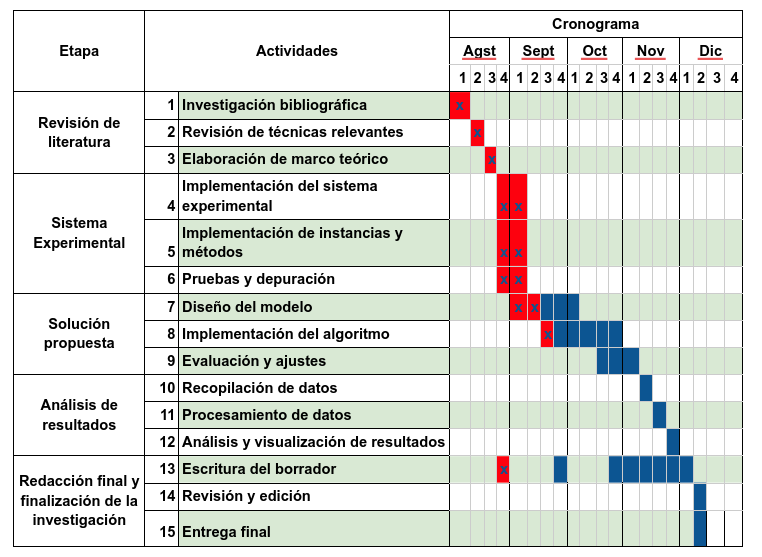
\includegraphics[width=1.1\linewidth]{Images/image.png}
%    \caption{Cronograma actual}
%    \label{fig:cronograma}
%\end{figure}
%\end{center}

%----------------Página de derechos de autor: elegir entre a) o b) y borrar/comentar la opción NO utilizada-----------------
\thispagestyle{empty}
\mbox{}                         % Ayuda a bajar el texto
\vfill                          % Deja el texto al fondo
\textcopyright\ 2023, José Ignacio González Cortés \\ % Derechos de autor
Se autoriza la reproducción total o parcial, con fines académicos, por cualquier medio o procedimiento, incluyendo la cita bibliográfica del documento
\vspace{1cm}    % lo separa del fondo
\restoregeometry % Devuelve los márgenes después de la portada


%----------------Página de calificaciones (opcional), descomentar para generar-----------------

% Editar en Otros -> Calificaciones.tex

%%Las calificaciones entregan la misma información de la portada y se le agrega la nota y la firma. Esta página es opcional.
\begin{titlepage}
	
	\newgeometry{top=1 in, bottom=1 in, left=1 in, right= 1 in} 
	
	\thispagestyle{frontpage}
	
	\begin{center}
		
		\vspace*{4\baselineskip}
	
		
		{\Huge \textbf{TÍTULO PRINCIPAL\\}}%No abreviar, no subrayar, no usar comillas. Se escribe completamente en mayúsculas
		        \vspace*{1.5\baselineskip}

		\large{\textit{subtítulo}}\\ %No abreviar, no subrayar, no usar comillas. Solo la priemra letra usa mayúsculas
		
        \vspace*{1,5\baselineskip}

		\large{\textbf{Por: Autor}}\\ %Nombre como aparece en registro académico
		
		\vspace{1,5\baselineskip}
		
		\large{Tesis presentada a la Facultad de Ciencias Físicas y Matemáticas de la Univerisdad de Concepción para optar al grado académico de Magister en Ciencias con Mención en Física.} %Cambiar a grado académico correspondiente. 
		
		\vspace{1,5\baselineskip}
		Diciembre 2019\\ %Mes y año de la tesis, solo primera letra del mes en mayúsculas
		Concepción, Chile %Ciudad y país de publicación.
\vspace{1,5\baselineskip}

		\large{\textbf{Profesor Guía: Nombre}}\\ %Nombre del profesor que dirigió el trabajo, de la comisión informante y otros asesores precedidos por los títulos correctos de la unidad académica.  
		%Al margen derecho del profesor guía se estampa la firma y/o calificación.
		

	\end{center}
	

	
\end{titlepage}         % Genera la pagina de calificaciones del archivo calificaciones.tex
%\restoregeometry                           % Devuelve los márgenes después de la página

%\pagenumbering{gobble}         % Suprime la numeración de páginas
%\thispagestyle{plain}          % suprime el encabezado
%\clearpage\mbox{}\clearpage    % Agrega página en blanco

%----------------Página de dedicatoria (opcional), descomentar para generar ---------------------------------


\thispagestyle{empty}
\mbox{}
\vfill
\hfill \text{Dedicatoria}

\restoregeometry

%-------------------------------------------------




%-----------------Página de agradecimientos (opcional), se incluye normalmente-------------------

% Editar en Otros -> Agradecimientos.

\pagenumbering{roman}                            % Empieza la enumeración romana en minúsculas, para mayúsculas usar Roman.


\newpage
\addcontentsline{toc}{chapter}{AGRADECIMIENTOS}  % Agrega esta sección al índice
\section*{AGRADECIMIENTOS}                       % Debe ir en mayúsculas por reglamento de la UdeC, tiene asterisco para no ser numerada.


\vspace*{2\baselineskip}

\lipsum[4-5] % Texto para mostrar la página, Borrar cuando se escriban los agradecimientos

\vspace*{3\baselineskip}




%-----------------Página de resumen (abstract)-------------

% Si la unidad académica lo requiere, se edita en  Otros -> Resumen.tex . El mismo resumen puede ser incluido en inglés (abstract) en la página siguiente, para agregarlo hay un espacio destinado en el mismo archivo antes mencionado.

\newpage
\addcontentsline{toc}{chapter}{Resumen} % Agrega esta sección al índice
\section*{Resumen}                      % Con asterisco para que no sea numerada.

    \par\vspace*{\fill} % Mueve las palabras clave al final de la página
    \textbf{\textit{Keywords --}} Knapsack Problem %Agregar todas las palabras claves asosciadas con la tesis aquí.
    
    %-----------Si se desea poner el Abstract Des-comentar lo siguiente-----------
    \newpage
    \addcontentsline{toc}{chapter}{Abstract} %Agrega esta sección al índice
    \section*{Abstract}
    
    \par\vspace*{\fill} % Mueve las palabras clave al final de la página
    \textbf{\textit{Keywords --}} Knapsack Problem % Agregar las palabras claves en inglés

%--------------Página de índice.  

%\nocite{*}     % Des-comentar si se desea que TODAS las referencias sean impresas en la lista de referencias, incluyendo las que no fueron finalmente citadas en el texto.

\newpage{\setstretch{1.0} \tableofcontents}
\newpage{\setstretch{1.0} \listoftables}
\newpage{\setstretch{1.0}\listoffigures}
\newpage{\setstretch{1.0}\listofalgorithms}

\newpage
\addtocontents{toc}{\protect\setcounter{tocdepth}{4}}   % La profundidad del índice queda en 4, 1.1.1.1
\pagenumbering{arabic}                                  % Comienza la numeración arábiga (números normales)
\setcounter{page}{1}                                    % Comienza el contador de páginas en 1

% A continuación se dejan nombres de diversos capítulos o secciones, para cambiar el nombre del archivo tan solo se debe hacer en la carpeta "capitulos" y luego llamarlos de la forma correcta en "\subfile{Capitulos/nuevonombre}".
% Los nombres de los archivos no pueden llevar tíldes ni espacios para el correcto funcionamiento del compilador, esto no tiene nada que ver con que tengan o no tilde en el documento final.

\chapter{Introducción}
Este capítulo presenta los antecedentes generales acerca del problema polinomial robusto de la mochila, las variantes de las cuales se deriva y metodologías de solución asociadas a estas. Además, los objetivos generales y específicos de esta memoria y la estructura del documento.


\section{Antecedentes generales}

El problema de la mochila (KP, por sus siglas en inglés, Knapsack Problem) es un problema clásico de la investigación de operaciones. Generalmente, el KP modela la necesidad de elegir un conjunto de elementos con costos y beneficios individuales, con una restricción de capacidad máxima, con el fin de maximizar el beneficio. El KP ha sido ampliamente estudiado por su estructura sencilla, y también debido a que muchos otros problemas de optimización más complejos lo tienen como subproblema \citep*{martello_knapsack_1990}.

El KP tiene muchas  variantes, una ellas es la versión robusta, RKP (por sus siglas en inglés, Robust Knapsack Problem). Esta fue formulada originalmente por \cite{eilon_application_1987} para resolver problemas de asignación de presupuesto con aplicaciones reales, el parámetro de costo del problema está asociado a incertidumbre. El RKP fue planteado para encontrar soluciones que sean factibles para todas las posibles variaciones en los costos de elementos \citep{monaci_exact_2013}.

Otra variante es la versión polinomial de la mochila (PKP, por sus siglas en inglés, Polynomial Knapsack Problem) que incluye el concepto de sinergias, es decir, que la elección de una o más alternativas específicas otorga un beneficio o costo extra según estas relaciones. El PKP sirve para modelar sistemas cuyas alternativas presentan conflictos entre ellas, o que cooperan para generar mayor beneficio \citep{baldo_polynomial_2023}. Así, de este problema surge el polinomial robusto (PRKP, por sus siglas en inglés, Polynomial Robust Knapsack Problem). El PRKP toma en cuenta costos inciertos y sinergias polinomiales para modelar problemas de selección de alternativas, que se perjudican o benefician entre sí y cuyos costos muestran comportamiento estocástico.

Debido a la dificultad para resolver el PRKP la literatura se ha limitado a explorar dos casos especiales del problema. El problema cuadrático de la mochila (QKP, por sus siglas en inglés, Quadratic Knapsack Problem) \citep{gallo_quadratic_1980} y el problema cúbico de la mochila (CKP, por sus siglas en inglés, Cubic Knapsack Problem) \citep{forrester_strengthening_2022}. El QKP presenta sinergias entre dos elementos y ha demostrado ser útil en un gran espectro de aplicaciones como posicionamiento satelital \citep{witzgall_mathematical_1975}, localizaciones de centros de transporte como aeropuertos, ferrocarriles o terminales de carga \citep{rhys_selection_1970}. El CKP es extendido desde el QKP y considera sinergias hasta con tres elementos. Además, posee aplicaciones como en el problema de satisfacción Max 3-SAT \citep{kofler_penalty_2014}, el problema de selección \citep{gallo_fast_1989}, el problema de alineación de redes \citep{mohammadi_triangular_2017}, y la detección y tratamiento de enfermedades de transmisión sexual \citep{zhao_treatments_2008}.

Este trabajo propone el uso de una técnica de machine learning para resolver el PRKP. Una estrategia greedy que descarte elementos de las soluciones para acotar el espacio, siendo escalable y rápida de ejecutar en grandes tamaños de instancias, usando una red neuronal para la toma decisiones. Se compara con la literatura y se analizan los resultados obtenidos en instancias conocidas con soluciones conocidas y desconocidas de mayor tamaño.

\section{Objetivos}
\subsubsection*{Objetivo general}
Implementar un algoritmo basado en machine learning para resolver el PRKP.
\subsubsection*{Objetivos específicos}
\begin{itemize}
	\item Revisar la literatura relacionada con problemas de la mochila similares y metodologías aplicables.
	\item Diseñar un algoritmo basado en machine learning para el PRKP.
	\item Implementar la estrategia propuesta basada en machine learning.
	\item Evaluar los resultados y comparar el rendimiento con las metodologías existentes en literatura.
\end{itemize}

\section{Estructura del documento}

El documento consta de seis capítulos, en los cuales se discute el problema y su formulación formal (2), la metodología propuesta para el PRKP (3), un análisis comparativo de los resultados experimentales (4), y finalmente, una revisión y discusión para concluir el documento (5).

\clearpage

\chapter{Problema Polinomial Robusto de la mochila}
Este capítulo comprende la definición formal del problema junto al modelo matemático de programación entera. Además, explora literatura asociada a técnicas y metodologías empleadas para la resolución de otros problemas de la mochila que pueden ser extendidos al PRKP.

\section{Descripción del problema}
	El PRKP es definido formalmente como un conjunto de elementos $I = \{1,2,\hdots,N\}$, donde estos tienen un beneficio asociado $P_i \in \mathbb{R}:i\in I$.Además, los elementos poseen un coste de comportamiento estocástico que puede variar de forma continua entre una cota inferior y una superior, $C_i \in [C^L_i,C^U_i]$, donde $C^L_i$ es el costo base, y $C^U_i$ el costo máximo. Solo algunos elementos tienen comportamiento estocástico, aquellos que no, cumplen que $C_i = C^L_i$. El parámetro que define cuantos elementos de $I$ pueden tener comportamiento estocástico es $\Gamma \leq |I|$, es decir $|\{i: C_i > C^L_i\}| \leq \Gamma$. Además, existe un presupuesto máximo $W$ para los costes. Mientras, el conjunto de sinergias polinomiales se define como $A = \{ \bar{I}_j \textbackslash \bar{I}_j \subseteq I: j \in 2^{|I|}\}$. Para cada sinergia $a \in A$ existe un beneficio asociado $P_a$. Finalmente, el objetivo del problema es encontrar $X \subseteq I$ que maximice el beneficio total de los elementos de $X$ sumado a los beneficios de sinergias, que aplican cuando $a \subseteq X$, y que además, mantenga un coste total menor al presupuesto para cualquier variación estocástica en costes de los elementos.
	
	Sea un ejemplo de instancia de PRKP con $I =\{1,2,3\},W = 10 \text{ y } \Gamma = 2$. La Tabla \ref{tab:example_p} describe las cotas inferior y superior de los costos de los elementos de la instancia, así como los beneficios de cada elemento individual. La Tabla \ref{tab:sinergias} muestra los beneficios de cada sinergia. El número de sinergias es siempre igual a $2^|I| - |I|$, aunque en el caso de que hayan sinergias cuyo beneficio es cero, estas se omiten de la tabla.	Una solución factible de esta instancia es $X = \{1,3\}$ cuyo beneficio total es 6, mientras que la solución óptima de esta instancia, es $X = \{2,3\}$ con un beneficio total de 9.
	
	\begin{table}[H]
		\centering
		
		\caption{Beneficios y costos de los ítems.}
		\label{tab:example_p}
	\begin{tabular}{|c|c|c|c|}
		\hline
		$i$ & 1 & 2 & 3 \\
		\hline
		$PS_i$ & 3 & 6 & 10 \\
		\hline
		$C^L_i$ & 2 & 3 & 4 \\
		\hline
		$C^U_i$ & 4 & 4 & 5 \\
		\hline
	\end{tabular}
	
	\end{table}
	
	\begin{table}[H]
		\centering
		\caption{Beneficios por sinergias.}
		\label{tab:sinergias}
		\begin{tabular}{|c|c|}
			\hline
			$A$    & $P_A$\\
			\hline
			$\{1,2\}$ & -2 \\
			\hline
			$\{1,3\}$ & 2 \\
			\hline
			$\{2,3\}$ & 2\\
			\hline
			$\{1,2,3\}$ & 3\\
			\hline
		\end{tabular}
	\end{table}
	

		

	
    
    \section{Modelo matemático}
    
    
    \cite{baldo_polynomial_2023} describe una formulación del PRKP mediante un modelo matemático linealizado que es compatible con solvers de propósito general. El modelo de programación lineal entera mixta (MILP) usa una variable de decisión binaria $x_i: i \in I$ que toma el valor 1 si un elemento pertenece a la solución final. Las variables de decisión $\rho$ y $\pi_i$ representan la diferencia entre el coste base y el coste máximo de un elemento. Se ajustan de forma que si el coste del elemento $i$ varía entonces la suma entre $\rho$ y $\pi_i$ es igual al coste máximo. Así la función objetivo se encarga de maximizar $\rho$ y $\pi_i$ para que considere el máximo coste posible para todos los elementos.
        
 \begingroup 
 \renewcommand{\arraystretch}{1.4}
  \begin{table}[H]
  \caption{Resumen de los conjuntos, parámetros y variables de decisión}
  \begin{tabular}{l p{11cm}}
  	\hline
  	Conjuntos & \\
  	\hline
  	$I$ & El conjunto de elementos \{ 1,2,\dots,N\}.\\
  	$A$& El conjunto de sinergias $\{ I_j \textbackslash I_j \subseteq I:j\in 2^|I| \}$.\\
  	\hline Parámetros & \\ \hline
  	
  	$P_i$ & El beneficio asociado al elemento $i \in I$. \\
  	$C^L_i$& El coste base del elemento $i \in I$.    \\
  	$C^U_i$& El coste máximo del elemento $i \in I$.     \\
  	$W$& El presupuesto o coste total máximo asociado al problema.\\
  	$B_a$ & El beneficio de la sinergia polinomial arbitraria $a \in A$.\\
  	$\Gamma$& El número máximo de elementos que pueden tener costo distinto al costo base.\\
  	
  	\hline Variables de decisión &\\ \hline
  	$x_i$ & Toma valor 1 si el elemento $i \in I$ está presente en la solución óptima.\\
  	$z_a$ & Toma valor 1 si $\forall a \in A, a \in X$, si no 0.\\
  	$\mathbb{\rho}, \mathbb{\pi}_i$ & Cumplen que  $\rho + \pi_i  = C_i^U - C_i^L$ si el coste del elemento $i$ varía, sino $\rho = C_i^U - C_i^L$ y $\pi_i = 0$.\\
  	\hline
  	
  \end{tabular}
  \end{table} 
  
  \endgroup
    
	
\begin{equation}
	\text{Maximizar} \quad \sum_{i\in I} P_i x_i + \sum_{a\in A} B_a z_a - \sum_{i\in I} LC_i x_i - \left(\Gamma\rho+\sum_{i\in I} \pi_i\right) \label{eq:of}
\end{equation}
\begin{align}	 
	&\sum_{i\in I} C_i^L x_i + \Gamma\rho + \sum_{i\in I} \pi_i \leq W& \label{eq:costs} \\
	&\rho + \pi_i \geq (C_i^U - C_i^L) x_i & \forall i \in I \label{eq:cost_relax} \\
	&\sum_{i\in a} x_i \leq |a| - 1 + z_a & \forall a \in A:B_a < 0 \label{eq:fijar_z} \\
	&z_a \leq x_i & \forall i \in a, \forall a \in A : B_a > 0 \label{eq:fijar_z_2} \\
	&x_i \in \{0,1\} \quad &\forall i \in I \\
	&z_a \in \{0,1\} \quad &\forall a \in A \\
	&\rho \in \mathbb{R}^{+} \quad \pi_i \in \mathbb{R}^{+} &\forall i \in I \label{eq:dom}
\end{align}
	

    
    La función objetivo \eqref{eq:of} representa el beneficio total de elementos y sinergias de los elementos restando el coste máximo posible que estos puedan tener. $\sum_{i\in I} P_i x_i$ es la suma de todos los beneficios individuales de cada elemento. $\sum_{a\in A} B_a z_a$ corresponde a la suma de los beneficios de cada sinergia $\sum_{i\in I} C_i^L x_i$ es la suma de todos los costes mínimos  y corresponde a la suma de la diferencia de los costes. $\left(\Gamma\rho+\sum_{i\in I} \pi_i\right)$. Las ecuaciones \eqref{eq:costs} y \eqref{eq:cost_relax} representan la restricción de presupuesto. La solución debe ser robusta a las variaciones en los costes por lo que se usa un acercamiento que asume el peor de los casos, es decir, el cálculo del coste es siempre maximizado según las posibles variaciones. Para ello \cite{baldo_polynomial_2023} genera el problema dual de la maximización de los costes, construyendo la dualidad de Lagrange. Esto resulta en las restricciones \eqref{eq:costs} y \eqref{eq:cost_relax} y las variables de decisión auxiliares $\rho$ y $\pi_i (i \in I)$, de forma que el cálculo del coste se expresa como un problema de minimización. Las restricciones \eqref{eq:fijar_z} y \eqref{eq:fijar_z_2} aseguran que el valor de $z$ estableciéndolo como uno si todos elementos de una sinergia están en la solución final y cero en caso contrario. La restricción \eqref{eq:dom} establece $\rho$ y $\pi_i$ números reales positivos, así el modelo no establece costes negativos en la función de maximización y en el cálculo del coste. A través de la restricción \eqref{eq:cost_relax}.
  
\section{Revisión de literatura}


El trabajo de \cite{baldo_polynomial_2023} introduce el PRKP y una metodología para resolverlo, proponiendo un algoritmo genético y un algoritmo basado en machine learning. Este último utiliza un clasificador random forest que predice la probabilidad de cada elemento de estar presente en la solución óptima. Esta predicción se usa para fijar variables de decisión, reduciendo así el tiempo de ejecución de un solver exacto. Como solo existe un trabajo para el PRKP, esta revisión se enfoca en metodologías de solución basadas en machine learning para variantes del KP. \cite{li_novel_2021} utiliza redes neuronales para obtener predicciones de soluciones para instancias de KP que poseen funciones objetivo no lineales desconocidas. De esta forma solo se conocen parcialmente algunos valores de la función objetivo pero no su formulación. Los autores obtienen buenos resultados con una estructura basada en teoría de juegos, junto al uso de redes neuronales adversarias, considerando una red para modelar la función objetivo y otra con el método de descenso de gradiente adaptativo para resolver el problema.

\cite{rezoug_application_2022} aborda el KP usando distintas técnicas para evaluar las características de los elementos, entre ellos redes neuronales, regresión de procesos gaussianos, random forest y support vector regression. Ellos resuelven el problema original usando solo un subconjunto de los elementos. Luego mediante el descenso del gradiente y el uso de características de los elementos deciden cuáles de los elementos excluidos debe agregar a la solución inicial obtenida. Los resultados muestran que el modelo machine learning entrega soluciones similares a los otros clasificadores y con menores tiempos de ejecución.

\cite{afshar_state_2020} propuso un algoritmo para generar soluciones para el KP usando un modelo de deep reinforcement learning que selecciona los elementos de forma greedy. El algoritmo propuesto construye las soluciones en base a las decisiones del modelo y genera soluciones con una razón de similitud con el óptimo del 99.9\%. Además, usa una arquitectura dos redes neuronales con un paso de reducción de dimensión de características que reduce la complejidad espacial del problema en la red. Esto resulta en modelos que usan menos memoria y se ejecutan más rápido.

El uso de técnicas basadas en machine learning para abordar variantes del KP en la literatura, evidencian la posibilidad de diseñar estrategias efectivas que resuelvan el PRKP de forma eficiente.
 

\chapter{Metodología}

Este capítulo presenta el algoritmo propuesto para resolver el PKRP, así como las definiciones del modelo de machine learning que actúa como clasificador, las características de los elementos que se usan y el proceso de reducción de instancias.

\section{Algoritmo propuesto}

Se propone un algoritmo iterativo con el objetivo de reducir la complejidad del problema de forma gradual, a costa del nivel de confianza sobre la solución final obtenida. El algoritmo usa una red neuronal como clasificador, que se basa en características de cada elemento para decidir la probabilidad de estar o no en la solución final. El clasificador es entrenado antes del algoritmo general para obtener predicciones adecuadas. Estas predicciones son usadas para que los elementos tomen valores de 0\% de probabilidad y así reducir la instancia original a una más pequeña. Este proceso es ejecutado un número arbitrario de veces, mientras se mantenga la precisión del modelo, al evaluar instancias con cada vez menos elementos. El enfoque define una estructura para la red, una serie de características para elemento, dos etapas de entrenamiento y un algoritmo de evaluación que usa el clasificador entrenado para evaluar y encontrar soluciones para las instancias.


La metodología se desarrolla en tres etapas fundamentales. En primer lugar, se crea y entrena un clasificador basado en una red neuronal. Este clasificador está diseñado para evaluar la probabilidad de que cada elemento pertenezca a la solución final del Problema de la Mochila Probabilística Restringida (PKRP). Las características específicas de cada elemento, como el costo normalizado, el rango de costos, la variabilidad estocástica y otros, se utilizan como entrada para el clasificador.

En la segunda etapa, se lleva a cabo el entrenamiento de la red neuronal en dos fases. Inicialmente, se entrena la red con soluciones óptimas generadas por un solver exacto para establecer un clasificador general. Posteriormente, se realiza una afinación más precisa utilizando pasos intermedios del algoritmo general propuesto.

Finalmente, en la tercera etapa, se emplea el clasificador entrenado en el algoritmo general de evaluación. Este algoritmo iterativo busca reducir gradualmente la complejidad del PKRP, utilizando el clasificador para predecir la probabilidad de inclusión de cada elemento en la solución final. Se realiza una reducción de instancias mediante la eliminación de elementos menos probables de contribuir a la solución, manteniendo la precisión del modelo a lo largo de las iteraciones. En resumen, la metodología abarca la creación y entrenamiento del clasificador, seguido de su utilización en el algoritmo iterativo para evaluar y reducir instancias del PKRP.



\begin{algorithm}[H]
	\caption{Algoritmo de evaluación}\label{alg:general}
	\begin{algorithmic}[1]
		\Statex \textbf{Input:} $\tau$
		\Statex \textbf{Output:} $x$
		\Loop
		\State $F \gets$ \texttt{F($I$)}\label{alg1:full_features}
		\State $\tilde{x} \gets$ \texttt{Net($F$)} \label{alg1:get_pred}
		\State $Z \gets$ \texttt{Z($I$,$\tilde{x},\tau$)} \label{alg1:get_Z}
		\If{$ |Z| = 0$ \textbf{or} $\min(\tilde{x}) > \tau$} \label{alg1:break_condition}
		\State \textbf{break}
		\EndIf
		\State $I \gets I\setminus Z$ 								\label{alg1:update_I}
		\State $S \gets \{A \in S, \forall i \in A: i \notin Z\}$  \label{alg1:update_S}
		\EndLoop
		\State $x \gets$ \texttt{Solver($I$)} \label{alg1:exact_solver} 
	\end{algorithmic}
\end{algorithm}



El Algoritmo \ref{alg:general} se encarga de usar una red pre-entrenada como clasificador y resolver la instancia. Comienza dentro de un ciclo, el primer paso en la línea \ref{alg1:full_features} es generar características derivadas de los parámetros del modelo, que describan a cada elemento en particular. Estas características son usadas por la red en la línea \ref{alg1:get_pred} para generar la predicción de cada elemento. El conjunto de elementos de la instancia, la predicción de la red y el parámetro $\tau$ son usados en la línea \ref{alg1:get_Z} para generar $Z$, el conjunto de elementos a eliminar de la solución final. $\tau$ define el mínimo valor que debe tener la predicción de un elemento, para ser ignorado en la solución final. Todos los elementos de $Z$ se quitan de la instancia, así como las respectivas sinergias polinomiales en las líneas \ref{alg1:update_I} y \ref{alg1:update_S}. Este proceso se ejecuta hasta que $Z$ se construye sin elementos, o hasta que ningún elemento consigue una probabilidad de ser cero menor a $\tau$. Finalmente, en la linea \ref{alg1:exact_solver} se usa un solver exacto para resolver la instancia que contiene un número reducido de elementos.



\newcommand{\algrule}[1][.2pt]{\par\vskip.5\baselineskip\hrule height #1\par\vskip.5\baselineskip}


\section{Clasificador}

El clasificador utilizado es una red neuronal de tres capas de 50 nodos cada una, con una salida, y una función de activación. Estructurada para tomar como entrada las características de un elemento y obtener la predicción.
	
	\begin{figure}[H]
		\centering
		\begin{tikzpicture}[scale=0.6]
			
			% Nodos de entrada
			\foreach \x in {2,...,7} {
				\node[shape=circle, draw=black] (Input\x) at (0,\x)  {};
			}
			
			% Nodos de la capa oculta
				\node[shape=circle, draw=black, scale=0.6] (Hidden13) at (2,3)  {48};
				\node[shape=circle, draw=black, scale=0.6] (Hidden12) at (2,2)  {49};
				\node[shape=circle, draw=black, scale=0.6] (Hidden11) at (2,1)  {50};
				\node[shape=circle, draw=black, scale=0.6] (Hidden23) at (5,3)  {48};
				\node[shape=circle, draw=black, scale=0.6] (Hidden22) at (5,2)  {49};
				\node[shape=circle, draw=black, scale=0.6] (Hidden21) at (5,1)  {50};
				\node[shape=circle, draw=black, scale=0.6] (Hidden32) at (8,2)  {48};
				\node[shape=circle, draw=black, scale=0.6] (Hidden33) at (8,3)  {49};
				\node[shape=circle, draw=black, scale=0.6] (Hidden31) at (8,1)  {50};
				\node[shape=circle, draw=black, scale=0.6] (Hidden17) at (2,6)  {3};
				\node[shape=circle, draw=black, scale=0.6] (Hidden18) at (2,7)  {2};
				\node[shape=circle, draw=black, scale=0.6] (Hidden19) at (2,8)  {1};
				\node[shape=circle, draw=black, scale=0.6] (Hidden27) at (5,6)  {3};
				\node[shape=circle, draw=black, scale=0.6] (Hidden28) at (5,7)  {2};
				\node[shape=circle, draw=black, scale=0.6] (Hidden29) at (5,8)  {1};
				\node[shape=circle, draw=black, scale=0.6] (Hidden37) at (8,6)  {3};
				\node[shape=circle, draw=black, scale=0.6] (Hidden38) at (8,7)  {2};
				\node[shape=circle, draw=black, scale=0.6] (Hidden39) at (8,8)  {1};
			
			
			% Nodo de salida
			\node[shape=circle, draw=black] (Output) at (11,4.5)  {};
			
			% Nodo de transformación
			\node[scale=1.5] (Transformation) at (13.7,4.5)  {$\tilde{x}$};
			
			% Conexiones en la capa de fondo
			\begin{scope}[on background layer]
				% Conecto la capa 2 con la 3
				\foreach \a in {1,2,3,7,8,9}{
					\foreach \b in {1,2,3,7,8,9}{
						\draw (Hidden2\a) to (Hidden3\b);}
				}
				
				% Conecto la entrada con la capa 1
				\foreach \x in {2,...,7}{
					\foreach \y in {1,2,3,7,8,9}{
						\draw (Input\x) to (Hidden1\y);
					}        
				}
				
				% Conecto la capa 1 con la capa 2
				\foreach \a in {1,2,3,7,8,9}{
					\foreach \b in {1,2,3,7,8,9}{
						\draw (Hidden1\a) to (Hidden2\b);}
				}
				
				% Conecto la capa 3 con la capa Salida
				\foreach \x in {1,2,3,7,8,9}{
					\draw (Hidden3\x) to (Output);        
				}
			\end{scope}
			
			% Conexión entre el nodo de salida y el nodo de transformación
			\draw (Output) to (Transformation);
			
			% Dots
			\node at (2,4.75) {\vdots};
			\node at (5,4.75) {\vdots};
			\node at (8,4.75) {\vdots};
			
			% Etiquetas
			\node at (-1.5,7) {$f_1(i)$};
			\node at (-1.5,6) {$f_2(i)$};
			\node at (-1.5,5) {$f_3(i)$};
			\node at (-1.5,4) {$f_4(i)$};
			\node at (-1.5,3) {$f_5(i)$};
			\node at (-1.5,2) {$f_6(i)$};
			
			\node at (-1,10) {Entrada};
			\node at (2,10) {Capa $1$};
			\node at (5,10) {Capa $2$};
			\node at (8,10) {Capa $3$};
			\node at (11,10) {Salida};
			
		\end{tikzpicture}
		\caption{Estructura general de la red neuronal.}
		\label{fig:network}
	\end{figure}


La Figura \ref{fig:network} muestra la entrada de la red neuronal como un vector que contiene todas las características del elemento $i \in I$ y genera un número en la capa de salida. La función de activación es tangente hiperbólica que se aplica a la capa de salida de la red para ajustar la predicción a al rango [-1,1]. Luego,la predicción para cada elemento está dada por la  transformación la Ecuación \eqref{eq:soltransformation}. 


\begin{equation}
	\tilde{x}(i) = \frac{1}{2}\left( \tanh(Out(i)) + 1 \right)
	\label{eq:soltransformation}	
\end{equation}


Así, la red toma como argumento el vector de características $\texttt{f($i$)} = \textbf{(}f_1(i),f_2(i),f_3(i),f_4(i),f_5(i),f_6(i)\textbf{)}$, para retornar $x_i$, la predicción para el elemento $i$, entre cero y uno. Además, se puede extender como en la Ecuación \eqref{eq:net_matrix} que toma como entrada una matriz $F(I)$ como  definida en la Ecuación \eqref{eq:feature_matrix} que contiene las características de todos los elementos y obtiene como resultado el vector $\tilde{x}$ que contiene las probabilidades $\tilde{x_i} (\forall i \in I)$, que sirve como predicción de solución para la instancia.

\begin{equation}
	\label{eq:net_vector}
	Net(f) = \tilde{x_i} \quad: f\in [0,1]^6 \rightarrow \tilde{x}_i \in[0,1]
\end{equation}

\begin{equation}
	\label{eq:net_matrix}
	Net(F) = \tilde{x}\quad: F\in [0,1]^{6\times |I|} \rightarrow x \in[0,1]^{|I|}
\end{equation}

\begin{equation}
	F(I) \in M_{6 \times |I|} = 
	\left( 
	\begin{matrix}
		f(1)\\
		f(2)\\
		\vdots \\
		f(|I|-1)\\
		f(|I|)\\
	\end{matrix}
	\right)
	\label{eq:feature_matrix}
\end{equation}


\begin{multicols}{2}
	\label{eq:all_features}
	\begin{equation}
		f_1\left(i\right)   = \frac{P_i}{W}
		\label{feature:1}
	\end{equation}
	
	\begin{equation}
		f_2\left(i\right)   = \frac{C^L_i}{W}
		\label{feature:2}
	\end{equation}
	
	\begin{equation}
		f_3\left(i\right)   = \frac{C^U_i}{W}
		\label{feature:3}
	\end{equation}
	
	\begin{equation}
		f_4\left(i\right)   = \frac{\Gamma}{|I|}
		\label{feature:4}
	\end{equation}
	
	\begin{equation}
		f_5\left(i\right)   = \text{ContSol}_i
		\label{feature:5}
	\end{equation}
	
\begin{equation}
	\label{feature:6}
	f_6(i) = \frac{|I|_{\text{Actual}}}{|I|_\text{Original}}
\end{equation}	
\end{multicols}






Entre estas:
\begin{itemize}
	\item La característica en la ecuación \eqref{feature:1}, representa el costo de un elemento normalizado al presupuesto total disponible para en la instancia del problema.
	\item Las ecuaciones \eqref{feature:2} y \eqref{feature:3}, son el costo base y el costo máximo respectivamente, normalizados usando el presupuesto.
	\item La característica de la ecuación \eqref{feature:4}, representa el porcentaje de los elementos que varían estocásticamente su coste. Es una característica agregada de todos los elementos de una instancia que es invariable del elemento.
	
	\item $ContSol_i$ se refiere a la solución de la relajación continua del PRKP en que la variable de decisión $x_i$ en el modelo de programación lineal es continua.
	
	\item La característica de la ecuación \eqref{feature:6} es un indicador de cuanto se ha reducido la instancia en cada iteración del Algoritmo \ref{alg:general}, tiene un valor de $1$ en la primera iteración y va decreciendo a medida que se eliminan elementos a considerar del conjunto $I$.
	
\end{itemize}


\subsection{Entrenamiento}

La primera etapa consiste en entrenar la red para predecir la solución óptima de cada instancia, y así crear un clasificador general. La segunta etapa afina la precisión usando de los pasos intermedios del algoritmo de evaluación (\ref{alg:general}). Además, la red se entrena con soluciones que son generadas por un solver exacto que calcula el óptimo para cada instancia. 

\begin{algorithm}[H]
	\caption{Entrenamiento}\label{alg:training}
	\begin{algorithmic}[1]
		\Statex \textbf{Salida} $\texttt{Net}$
		\label{line:loss}
		\State $\texttt{Net}$ \label{line:def_net}
		\For{Instance $\in$ TrainingSet}   \label{line:startloop}
		\State $I \gets Instance$ \label{line:i_from_instance}
		\State $x \gets \texttt{Solver}(I)$\label{line:solveinstance}
		\For{$i \in I$} \label{line:startinnerloop}
		\State $\tilde{x_i} \gets \texttt{Net}(\texttt{f}(i))$   \label{line:prediction}
		\State $loss \gets \texttt{Loss}(x_i,\tilde{x_i})$ \label{line:calculateloss}
		\State $Net \gets \texttt{Optimizer(Net,$loss$)}$ \label{line:optimizationstep}
		\EndFor \label{line:endinnerloop}
		\EndFor \label{line:endloop}
	\end{algorithmic}
\end{algorithm}

El Algoritmo \ref{alg:training} de entrenamiento comienza inicializando la red con pesos aleatorios en la línea \ref{line:def_net}. A continuación, se inicia un bucle itera sobre cada instancia del conjunto de entrenamiento en la línea \ref{line:startloop}. Para cada instancia, se obtiene el conjunto de elementos $I$ de la instancia, en la línea \ref{line:i_from_instance}. Se obtiene la solución óptima $x$ para la instancia usando el solver en la línea \ref{line:solveinstance}. Posteriormente, se inicia un ciclo interno sobre los elementos de la instancia, donde la red neuronal realiza predicciones $\tilde{x_i}$ sobre las características de cada elemento utilizando la función \(f(i)\) en la línea \ref{line:prediction}.
Usando esta predicción se calcula la perdida entre la solución real $x_i$ y la predicción $\tilde{x}_i$ del elemento. Los pesos de la red se actualizan usando el algoritmo de optimización Adam, introducido por \cite{kingma2017adam}, que funciona como alternativa al descenso de gradiente estocástico, usando la pérdida anteriormente calculada. El proceso de predicción, cálculo de pérdida y optimización se repite para todos los índices en el bucle interno. Una vez completado, se regresa al bucle externo para la siguiente instancia del conjunto de entrenamiento. Habiendo procesado todas las instancias del conjunto de entrenamiento, la red neuronal $Net$ se considera entrenada y el algoritmo termina.

\begin{algorithm}[H]
	\caption{Afinación}\label{alg:tunning}
	\begin{algorithmic}[1]
		\Statex \textbf{Input: $\tau$ \texttt{Net}}
		\Statex \textbf{Output: \texttt{Net}}
		\For{Instance $\in$ TrainingSet}
				\State $I \gets \text{Instance}$ \label{line:def_I}
				\Loop
					\State $\tilde{x} \gets \texttt{Net}(F(I))$   \label{line:alg2:initial_pred}
					\State $Z \gets \texttt{Z($I,\tilde{x},\tau$)}$ \label{start_reduction_alg}
					\If{$ |Z| = 0$ \textbf{or} $\min(\tilde{x}) > \tau$ }
						\State $\textbf{break}$ 
					\EndIf
					\State $I \gets I\setminus Z$ \label{alg1:update_I_2}
					\State $S \gets \{A \in S, \forall i \in A: i \notin Z\}$  \label{end_reduction_alg}
				\State $x \gets \texttt{Solver}(I)$   \label{solve_smaller}
				\State $\tilde{x} \gets \texttt{Net}(F(I))$  \label{pred_smaller}
			\For{$i \in I$}
				\State $loss \gets \texttt{Loss($x_i,\tilde{x_i})$}$ \label{smaller_loss}
				\State $\texttt{Net} \gets \texttt{Optimizer}(\texttt{Net},loss)$	  \label{smaller_optim}
			\EndFor
			\EndLoop
		\EndFor
	\end{algorithmic}
\end{algorithm}

El Algoritmo \ref{alg:tunning} describe la etapa de afinación y sigue una estructura similar a la del Algoritmo \ref{alg:general}. El ciclo principal itera sobre instancias del conjunto de entrenamiento y define el conjunto de elementos de la instancia en la linea \ref{line:def_I}. La instancia es sujeta al proceso de reducción del Algoritmo \ref{alg:general} entre las lineas \ref{line:alg2:initial_pred} y \ref{end_reduction_alg}. Al finalizar cada reducción se obtiene la solución óptima de la instancia reducida y la predicción de la red en las líneas \ref{solve_smaller} y \ref{pred_smaller}. La solución óptima y la predicción de la red son usadas para calcular la perdida de cada elemento de la instancia reducida y actualizar los pesos de la red usando el algoritmo de optimización Adam. Este proceso afina la red para mejorar su precisión en instancias que han sido generadas por la reducción. Al finalizar la reducción y entrenamiento consecutivos con cada instancia del conjunto de entrenamiento, la red se encuentra entrenada para su uso en el Algoritmo \ref{alg:general} de evaluación.


 \section{Reducción de instancias}
 
 
 El proceso de reducción descrito en el Algoritmo \ref{alg:general} requiere definir el proceso de creación de Z con base en los parámetros. El Algoritmo \ref{alg:z} construye Z de forma que contenga los elementos ordenados con predicciones mas cercanas a cero que estén bajo el umbral $\tau$, con un tamaño máximo de $\mu$. Comienza estableciendo el tamaño maximo de $Z$, $\mu$, que se calcula como el numero de elementos de la instancia, divido sobre su magnitud. Si la instancia posee 10.000 elementos,como maximo $Z$ tendrá 2.500. Luego se crea el conjunto $B$ que posee todos los elementos cuya predicción $\tilde{x}_i$ es menor que $\tau$ en la línea \ref{create_B}. Luego en la línea  \ref{sort_b} B es ordenado de manera ascendente, de forma que $\tilde{x}_{B_b} < \tilde{x}_{B_{b+1}}   \forall b \in [1,|B|]$. Así, en un bucle que itera sobre los elementos ordenados de B, estos son agregados a Z en la linea \ref{add_to_z}. Este ciclo termina cuando B se queda sin elementos que agregar, o si la cardinalidad de Z supera el número máximo elementos definido por $\mu$.
 
    \begin{algorithm}[H]
 	\caption{$Z(I,\tilde{x},\tau)$}\label{alg:z}
 	\begin{algorithmic}[1]
 		\Statex \textbf{Input:} $I$,$\tilde{x}$,$\tau$
 		\Statex \textbf{Output:} Z
 		\State $\mu \gets \frac{|I|}{\log_{10}{|I|}}$ \label{alg2:def_mu} 
 		\State $B \gets \{ i \in I: \tilde{x}_i \leq \tau \}$ \label{create_B}
 		\State $B \gets \mathtt{Sort}(B)$  \label{sort_b}
 		\State $Z \gets \{\}$	  
 		
 		\ForAll{$b \in B$}
 		\State $Z \cup \{b\} $ \label{add_to_z}
 		\If{$|Z| = \mu$}\label{if_c}
 		\State \textbf{break} \label{break}
 		\EndIf
 		\EndFor
 	\end{algorithmic}
 \end{algorithm}
 
 
 
 
\clearpage
\chapter{Resultados Experimentales}
Este capítulo se presenta la comparación cuantitativa de los métodos de la literatura y el método propuesto.

\section{Instancias}

Las instancias provienen de un generador implementado por \cite{baldo_polynomial_2023} cuyas sinergias tienen en su mayoría beneficios de cero. Las instancias con $I$ mayor a 1000, tienen una generación exponencial de sinergias (|S| $\sim$ $aI^{a|I|}$). Para $300 \le I \le 1000$, se usa una generación cuadrática de sinergias (|S| $\sim$ $aI^{2}$). Para instancias con menos de 300 elementos, se generan sinergias de forma lineal (|S| $\sim$ $a|I|$).

Para comparar el rendimiento del algoritmo propuesto con los métodos de \cite{baldo_polynomial_2023} se usa el mismo conjunto de instancias de sus experimentos. Además, se generan 50 nuevas instancias con $|I| = 20000$ con el objetivo de comparar rendimiento para problemas de un orden de magnitud más grande entre BaldoML y el método propuesto.

\section{Software y Hardware}

La implementación del algoritmo se desarrolló usando Python 3.11.6, usando como librerías principales Pytorch 2.1, Numpy 1.26, y Gurobipy como binding para Gurobi 10.0.3. Los resultados fueron calculados en Linux 6.6.8 en un Intel i7-8550U de 4 núcleos, 8 hilos a 4.2 Ghz y 32 GB de RAM. La implementación se encuentra disponible en \href{https://github.com/elMixto/PRKP.git}{Github} (https://github.com/elMixto/PRKP).

\section{Comparaciones}


Se calcularon los resultados para todas las instancias de \cite{baldo_polynomial_2023}, usando los métodos BaldoGA, BaldoML y el algoritmo propuesto usando $\tau \in \{0.05,0.1,0.15,0.2,0.25 \}$.


\subsection*{Resultados de entrenamiento}

Para entrenar el clasificador se usaron 2500 instancias provenientes del generador de \cite{baldo_polynomial_2023}. Estas tienen tamaños que varían entre 100 y 1500 elementos de forma no uniforme y con $\Gamma$ establecido de forma aleatoria entre cero y el numero elementos de cada instancia. El proceso de optimización se realizó 2 veces por cada instancia usando un learning rate de $10^{-5}$.


\begin{figure}[h]
	\centering
			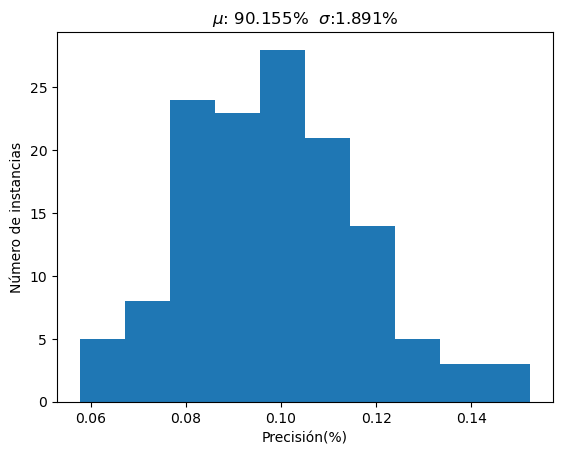
\includegraphics[scale=0.75]{graphs/training_performance.png}
	\caption{Distribución de la precisión del clasificador sobre instancias de evaluación}
	\label{fig:model_performance}
\end{figure}

La Figura \ref{fig:model_performance} muestra los resultados del entrenamiento. Se aplicó el modelo a un conjunto de evaluación de 135 instancias con tamaños entre 100 y 2000 elementos con $\Gamma$ aleatorio, alcanzando una precisión de 90,155\% con una desviacion estandar de 1,891\%. Es decir, en promedio, el clasificador puede predecir correctamente si un elemento está o no en la solución final de una instancia, un 90\% del tiempo.


\subsection*{Resultados generales}

La Figura \ref{fig:full_gap} presenta la distribución del Gap(\%) de cada método.
 BaldoGA tiene un gap promedio de $3,29\%$ y BaldoML tiene un gap promedio del 2,1\%. Estos resultados son congruentes con el estudio de \cite{baldo_polynomial_2023}, mostrando comparabilidad con los resultados. El método propuesto muestra un aumento en la variación del Gap(\%) conforme $\tau$ varía entre 0,05 y 0,25. Sin embargo, $\tau=0.05$ muestra una distribucion con menor media y variacion del Gap(\%) que a BaldoML y BaldoGA en todas las instancias. Respecto a los tiempos de ejecución. Por otro lado, la Figura \ref{fig:full_timegap} describe el TimeGap(\%) de los métodos usados, en los que el tiempo de ejecución está normalizado usando el tiempo de solucion del solver exacto. BaldoGA posee el peor rendimiento de los metodos, consiguiendo gaps mas altos y usando en mucho mas tiempo que el resto de métodos. El método propuesto con $\tau = 0.05$ no supera el 40\% del tiempo que tardó el solver.


\begin{figure}[H]
	\centering
	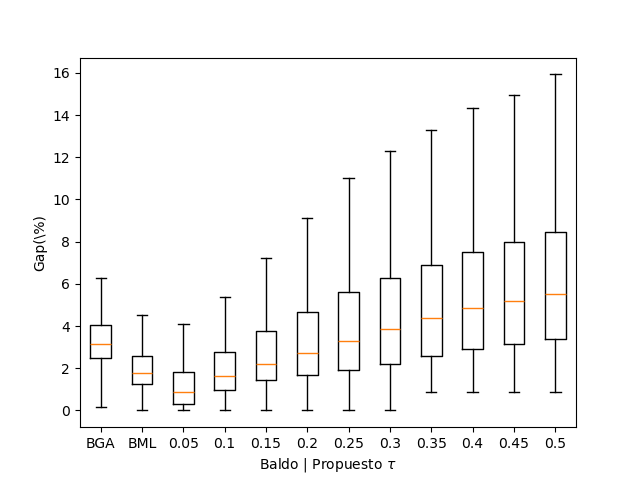
\includegraphics[scale=0.7]{graphs/full_gap_comparison.png}
	\caption{Distribución del Gap(\%) de cada método presentado}
	\label{fig:full_gap}
\end{figure}

\begin{figure}[H]
	\centering
	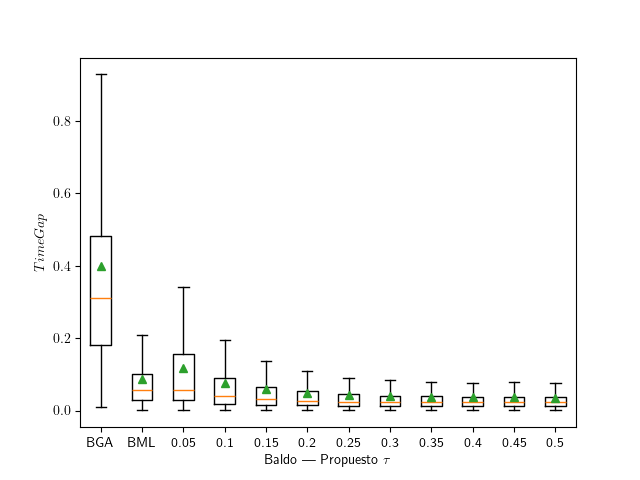
\includegraphics[scale=0.7]{graphs/full_timegap_comparison.png}
	\caption{Gap Tiempo(\%) de los métodos usados.}
	\label{fig:full_timegap}
\end{figure}


\begin{table}[H]
	\caption{Comparación general por número de elementos}
	\label{tab:general_comparison}
	\begin{adjustbox}{width=\columnwidth,center}
		\begin{tabular}{cccccccccccc}
			\multicolumn{3}{c}{Método} & &\multicolumn{8}{c}{|I|}\\
			\cline{1-3} \cline{5-12}
			\multicolumn{3}{c}{} & & 100  & 300  & 500  & 700  & 900  & 1100 & 1300 & 1500\\
			\hline
			\multirow{4}{*}{BaldoGA} & \multirow{2}{*}{Gap(\%)} & $\mu$ & & 1.74 & 3.07 & 3.04 & 3.42 & 3.74 & 3.4 & 4.1 & 3.9 \\
			& & $\sigma$ & & 1.15 & 0.905 & 0.866 & 0.844 & 1.09 & 1.07 & 6.89 & 1.18 \\
			\cline{2-3}
			& \multirow{2}{*}{Time(s)} & $\mu$ & & 0.44 & 3.3 & 4.5 & 7.18 & 9.86 & 5.61 & 7.22 & 8.89 \\
			& & $\sigma$ & & 0.207 & 1.32 & 1.75 & 2.93 & 4.08 & 2.19 & 2.44 & 3.21 \\
			\hline		 	 
			\multirow{4}{*}{BaldoML} & \multirow{2}{*}{Gap(\%)} & $\mu$ & & 3.16 & 3.0 & 2.2 & 2.0 & 1.85 & 1.41 & 1.37 & 1.39 \\
			& & $\sigma$ & & 1.87 & 1.19 & 0.907 & 0.722 & 0.659 & 0.56 & 0.592 & 0.497 \\
			\cline{2-3}
			& \multirow{2}{*}{Time(s)} & $\mu$ & & 0.0988 & 0.36 & 0.48 & 0.791 & 1.19 & 1.5 & 2.12 & 2.85 \\
			& & $\sigma$ & & 0.0147 & 0.0577 & 0.119 & 0.277 & 0.47 & 0.881 & 1.33 & 1.67 \\
			\hline		 						 
			\multirow{4}{*}{$\tau=0.05$} & \multirow{2}{*}{Gap(\%)} & $\mu$ & & 2.45 & 1.8 & 1.37 & 1.4 & 1.41 & 1.4 & 1.23 & 1.02 \\
			& & $\sigma$ & & 2.51 & 1.71 & 1.35 & 1.36 & 1.38 & 1.38 & 1.28 & 1.16 \\
			\cline{2-3}
			& \multirow{2}{*}{Time(s)} & $\mu$ & & 0.209 & 0.971 & 1.6 & 2.77 & 4.26 & 3.74 & 5.04 & 6.72 \\
			& & $\sigma$ & & 0.0997 & 0.392 & 1.17 & 2.07 & 3.27 & 2.97 & 3.72 & 4.72 \\
			\hline		 						        
			\multirow{4}{*}{$\tau=0.1$} & \multirow{2}{*}{Gap(\%)} & $\mu$ & & 4.35 & 3.26 & 2.82 & 2.74 & 2.69 & 2.43 & 2.34 & 2.12 \\
			& & $\sigma$ & & 3.32 & 2.19 & 1.89 & 1.96 & 1.86 & 1.67 & 1.72 & 1.59 \\
			\cline{2-3}
			& \multirow{2}{*}{Time(s)} & $\mu$ & & 0.164 & 0.772 & 1.03 & 1.57 & 2.46 & 2.16 & 2.95 & 3.68 \\
			& & $\sigma$ & & 0.0658 & 0.249 & 0.547 & 0.879 & 1.89 & 1.58 & 2.31 & 2.85 \\
			\hline		 						        
			\multirow{4}{*}{$\tau=0.15$} & \multirow{2}{*}{Gap(\%)} & $\mu$ & & 5.83 & 4.58 & 3.94 & 3.75 & 3.8 & 3.33 & 3.26 & 3.04 \\
			& & $\sigma$ & & 3.39 & 2.58 & 2.2 & 2.18 & 2.24 & 1.89 & 1.96 & 1.68 \\
			\cline{2-3}
			& \multirow{2}{*}{Time(s)} & $\mu$ & & 0.139 & 0.686 & 0.843 & 1.27 & 1.89 & 1.66 & 2.1 & 2.54 \\
			& & $\sigma$ & & 0.038 & 0.212 & 0.349 & 0.564 & 1.19 & 1.01 & 1.33 & 1.55 \\
			\hline		 						        
			\multirow{4}{*}{$\tau=0.2$} & \multirow{2}{*}{Gap(\%)} & $\mu$ & & 6.94 & 5.92 & 4.9 & 4.58 & 4.7 & 4.11 & 4.05 & 3.96 \\
			& & $\sigma$ & & 3.69 & 2.91 & 2.33 & 2.24 & 2.42 & 2.05 & 2.03 & 1.85 \\
			\cline{2-3}
			& \multirow{2}{*}{Time(s)} & $\mu$ & & 0.131 & 0.622 & 0.744 & 1.1 & 1.53 & 1.39 & 1.69 & 2.03 \\
			& & $\sigma$ & & 0.0234 & 0.135 & 0.26 & 0.393 & 0.676 & 0.675 & 0.86 & 0.999 \\
			\hline		 						        
			\multirow{4}{*}{$\tau=0.25$} & \multirow{2}{*}{Gap(\%)} & $\mu$ & & 7.84 & 6.84 & 5.76 & 5.42 & 5.54 & 4.81 & 4.84 & 4.84 \\
			& & $\sigma$ & & 3.95 & 3.04 & 2.37 & 2.28 & 2.46 & 2.15 & 2.07 & 1.99 \\
			\cline{2-3}
			& \multirow{2}{*}{Time(s)} & $\mu$ & & 0.126 & 0.596 & 0.685 & 0.974 & 1.32 & 1.2 & 1.44 & 1.68 \\
			& & $\sigma$ & & 0.0151 & 0.106 & 0.182 & 0.215 & 0.387 & 0.383 & 0.497 & 0.51 \\
		\end{tabular}
	\end{adjustbox}
\end{table}

El método propuesto con $\tau = 0.05$ muestra un menor Gap en comparación con BaldoML y BaldoGA en todos los tamaños de instancias. Esto indica que el método propuesto tiene un mejor rendimiento en términos de calidad de la solución obtenida. Aunque tiene tiempos de ejecución ligeramente más altos en comparación con BaldoML, la diferencia podría considerarse moderada. En todos los casos la desviación estándar de los tiempos de ejecución del algoritmo propuesto aumenta con la complejidad del problema de forma más rápida que BaldoML. Las instancias de 100 elementos poseen gaps particularmente mas altos para el método propuesto y BaldoML, para luego estabilizarse en instancias más grandes.


\begin{figure}[H]
	\centering
	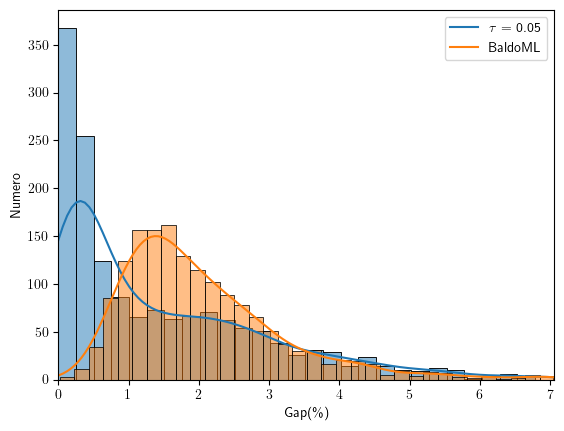
\includegraphics[scale=0.7]{graphs/distributions.png}
	\caption{Contraste distribución gap BaldoML vs Propuesto}\label{fig:distributions}
\end{figure}

El histograma de la Figura \ref{fig:distributions} ilustra la principal diferencia entre BaldoML y el propuesto. Los métodos tienen un gap medio de 2.05\% y 1.51\% respectivamente, esta diferencia de 0.54\% es significativa con un $p = 1.8\cdot10^{-26} < 0.05$ en una prueba T-student, rechazando la hipótesis de igualdad de medias. El método propuesto concentra una mayor proporción de instancias en gaps inferiores al 1\% que BaldoML .

\begin{figure}[H]
	\centering
	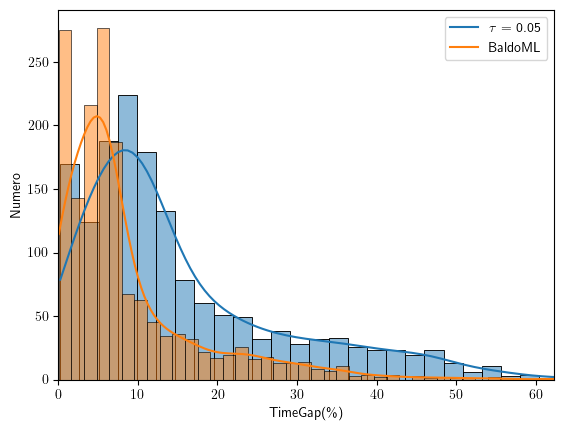
\includegraphics[scale=0.7]{graphs/distributions_times.png}	
	\caption{Contraste distribución tiempos de ejecución normalizados BaldoML vs Propuesto}\label{fig:distributions_times}
\end{figure}

Respecto a los tiempos de ejecución, BaldoML resolvió todas las instancias en 1859.86 segundos, lo que corresponde a 1.1719s en promedio por instancia. Mientras que el método propuesto tardó 4611.1s, con un promedio de 2.9 segundos. Debido a que las instancias tienen distintos tamaños y los tiempos de ejecución varían exponencialmente según este, se presenta en la Figura \ref{fig:distributions_times} una distribución de los tiempos normalizados. Ambas curvas se distribuyen de forma similar, con un desplazamiento positivo de la media del método propuesto, resultando en que una porción más alta de las instancias cae en TimeGaps de mayor magnitud. En promedio BaldoML se tarda 8.5\% del tiempo de gurobi en encontrar una solución, mientras que el propuesto un 15.93\%.



\subsection*{Instancias grandes}


Debido a la inviabilidad de utilizar el solver exacto para estos tamaños, las 50 instancias de $|I| = 20.000$ se resolvieron usando los métodos BaldoML y el propuesto para ser comparados de forma directa. Además, en estos tamaños el clasificador demuestra ser inviable con un $\tau = 0,05$. Al enfrentarse a tamaños con los que no fue entrenado, entrega predicciones de menor confianza, es decir más lejanas a cero, resultando en que el algoritmo no elimina ningún elemento. Relajar $\tau$ a un valor de $0,25$ resuelve este problema satisfactoriamente.

\begin{figure}[H]
	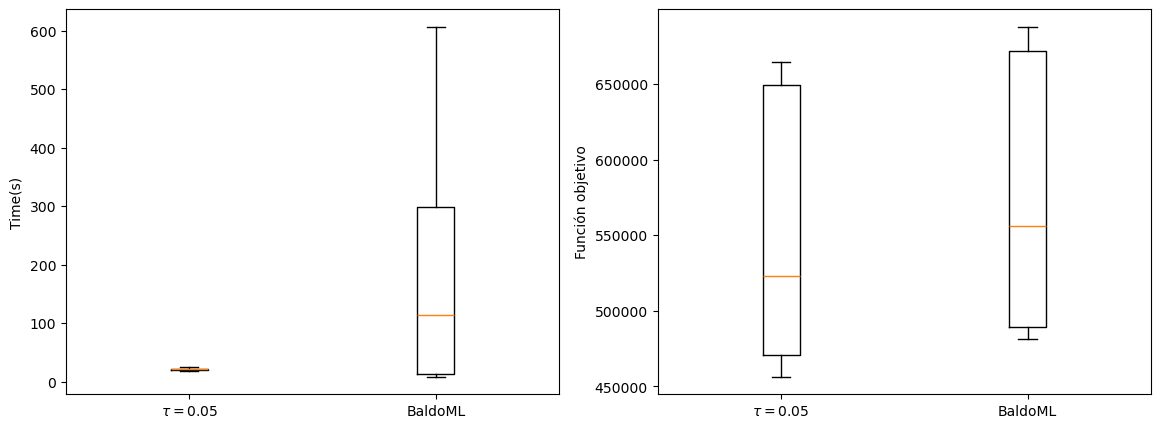
\includegraphics[scale=0.5]{graphs/comparison.png}	
	\caption{Comparación BaldoML y Propuesto en instancias de 20.000 elementos}
	\label{fig:comparison}
\end{figure}

En todos las instancias BaldoML encontró mejores soluciones, pero como se ilustra en la Figura \ref{fig:comparison} la diferencia entre esos es marginal. Las soluciones del método propuesto fueron en promedio un 4,47\% más pequeñas que las soluciones obtenidas por BaldoML, variando entre un 6,2\% y 2,85\% en el peor y mejor de los casos respectivamente. En cuanto a los tiempos de ejecución, la diferencia ha tenido mayor magnitud. Se estableció un límite de ejecución de 600 segundos por instancia. Mientras que BaldoML tardo 2 horas y 26  minutos en resolver las 50 instancias, el método propuesto usó poco menos de 18 minutos. Su tiempo de ejecución se mantiene relativamente constante en estos tamaños, mientras los tiempos de BaldoML se distribuyen de forma más amplia, con una desviación estándar muy alta.

\begin{table}[H]
	\centering
	\caption{Estadísticas, tiempos de ejecución en instancias grandes}
	\begin{tabular}{|c|c|c|}
		\hline
		&BaldoML& Propuesto\\
		\hline
		Tiempo total & 8.809s & 1.064,02s\\
		\hline
		Tiempo promedio &176,18s & $21.28s$ \\
		\hline
		Desviación estándar &164,44s& $1.60s$\\
		\hline
	\end{tabular}
\end{table}


\chapter{Conclusiones}
Esta memoria de título propone un algoritmo basado en machine learning para abordar el problema polinomial robusto de la mochila, usando un clasificador que opera de forma iterativa sobre una instancia para reducir su complejidad. Se ha definido la estructura de la red neuronal, el algoritmo general de operación, los 2 métodos de entrenamiento y el método de reducción de la instancia.
 
En los resultados, el algoritmo propuesto muestra un rendimiento objetivamente superior al algoritmo genético propuesto por \cite{baldo_polynomial_2023} en términos de precisión y tiempos de ejecución.Y Presenta mejores soluciones que BaldoML a pesar de tener tiempos de ejecución ligeramente mayores. Además, con una variación en los parámetros, tiene mejores características de escalamiento para abordar tamaños mayores a los contemplados en entrenamiento y evaluación. La metodología propuesta es entonces más adecuada para abordar instancias infactibles de resolver con un solver exacto, o con BaldoML en tiempos razonables.

En el futuro podría sería importante explorar el uso de técnicas más avanzadas de machine learning para abordar el problema. Implementar sistemas de decisión automática para los parámetros de los solvers mostrados y además explorar el uso de características derivadas de estimadores basados en machine learnig, como la arquitectura A2C introducida por \cite{mnih_asynchronous_2016}, con el fin de predecir características sin necesidad de derivarlas de la solución óptima.




    
    
\clearpage

\newpage
\renewcommand\refname{Referencias}          % Nombre para la lista de referencias, también se utiliza "Bibliografía"
{\setstretch{1.0}                           % Interlineado de las referencias 
\addcontentsline{toc}{chapter}{Referencias} % Cambia el nombre de la lista de referencias en el índice 
\bibliography{Referencias.bib}              % Agrega las referencias al documento, estas se ubican en el archivo Referencias.bib
}

\newpage
\renewcommand{\appendixpagename}{Apéndices}     % Nombre al inicio.
\addcontentsline{toc}{chapter}{Apéndices}       % Agrega "Apéndices" al índice





\end{document} 
